\chapter{Исследовательский раздел}

\section{Метрики оценки качества модели}

Поскольку задача обнаружения фальсифицированного фрагмента на изображении формулируется как задача сегментации на уровне пикселей, оценка качества модели должна учитывать как классификационную точность, так и пространственное соответствие предсказанных и истинных областей сфальсифицированного. В связи с этим для оценки качества метода используется комплекс метрик, специализированных для задач локализации аномалий.

Базой для вычисления всех показателей служат следующие понятия, определяемые на уровне каждого пикселя тестовой выборки:
\begin{itemize}[label = ---]
    \item TP (англ. True Positive) --- количество пикселей, корректно классифицированных как принадлежащих области сфальсифицированных;
    \item TN (англ. True Negative) --- количество пикселей, корректно классифицированных как принадлежащих фону;
    \item FP (англ. False Positive) --- количество пикселей, ошибочно отнесённых к области сфальсифицированных;
    \item FN (англ. False Negative) --- количество пикселей области сфальсифицированных, пропущенных моделью.
\end{itemize}

Точность на уровне пикселей отражает долю правильно классифицированных пикселей от общего числа пикселей в тестовой выборке:

\begin{equation}
    Accuracy = \frac{TP + TN}{TP + TN + FP + FN}.
\end{equation}

Данная метрика удобна для общей оценки, однако при сильном дисбалансе классов (область подделки обычно занимает менее 5-10 \% площади изображения) она может давать завышенные результаты за счёт доминирования класса фона.

Для более объективной оценки качества выделения целевой области используются точность (Precision) и полнота (Recall):
\begin{equation}
    Precision = \frac{TP}{TP + FP}.
\end{equation}
\begin{equation}
    Recall = \frac{TP}{TP + FN}.
\end{equation}

На основе этих показателей вычисляется F1-мера, представляющая собой гармоническое среднее точности и полноты:
\begin{equation}
    F1 = 2 \cdot \frac{Precision \cdot Recall}{Precision + Recall} = \frac{TP}{TP + \frac{1}{2} (FP + FN)}.
\end{equation}

F1-мера устойчива к дисбалансу классов и широко применяется в задачах обнаружения локальных артефактов, поскольку учитывает как пропущенные ложные пиксели, так и ложные срабатывания на фоне. 

Ключевой метрикой пространственного соответствия является коэффициент пересечения над объединением (англ. Intersection over Union, IoU):
\begin{equation}
    IoU = \frac{TP}{TP+FP+FN}.
\end{equation}

IoU измеряет степень перекрытия предсказанной маски подделки с эталонной разметкой и является стандартом де-факто в задачах сегментации. Значение IoU = 1 указывает на идеальное совпадение границ, а IoU=0 --- на полное отсутствие пересечения.

Все метрики вычисляются на уровне пикселей для каждой тестовой пары «изображение -- маска», после чего усредняются по всей тестовой выборке. Такой комплексный подход (F1-мера и IoU) обеспечивает всестороннюю оценку способности сверточной нейронной сети локализовывать фальсифицированные фрагменты при различных объёмах и конфигурациях входных данных. В дальнейшем эти две метрики будут использоваться как основные для анализа результатов всех экспериментов.

\section{Влияние слоя внимания на качество модели}

Целью данного исследования является изучение эффективности использования слоев внимания в реализованной модели сверточной нейронной сети. 

Для проведения этого исследования было выполнено сравнительное тестирование двух конфигураций модели: с использованием слоев внимания и без них. Все остальные компоненты архитектуры оставались неизменными. Эксперимент проводился на одной и той же тестовой выборке, что обеспечило объективность сравнения. Результаты эксперимента представлены в таблице \ref{tab:seam}.

\begin{table}[H]
    \centering
    \caption{Зависимость точности от конфигураций}\label{tab:seam}
    \begin{tabular}{|p{5.5cm}|p{4cm}|p{4cm}|}
		\hline
     \textit{Конфигурация} & \textit{{Значение F1}} & \textit{Значение IoU}\\ \hline
	\centering C использованием слоев внимания &  0.9042 &  0.8252 \\ \hline
    \centering Без использования слоев внимания &  0.6784 &  0.5133 \\\hline
    \end{tabular}
\end{table}

Примеры результатов обнаружения модели при различных конфигурациях слоев внимания представлены на рисунке \ref{img:seam1}.

\captionsetup{justification=centering,singlelinecheck=off}
\begin{figure}[h!]
    \centering
        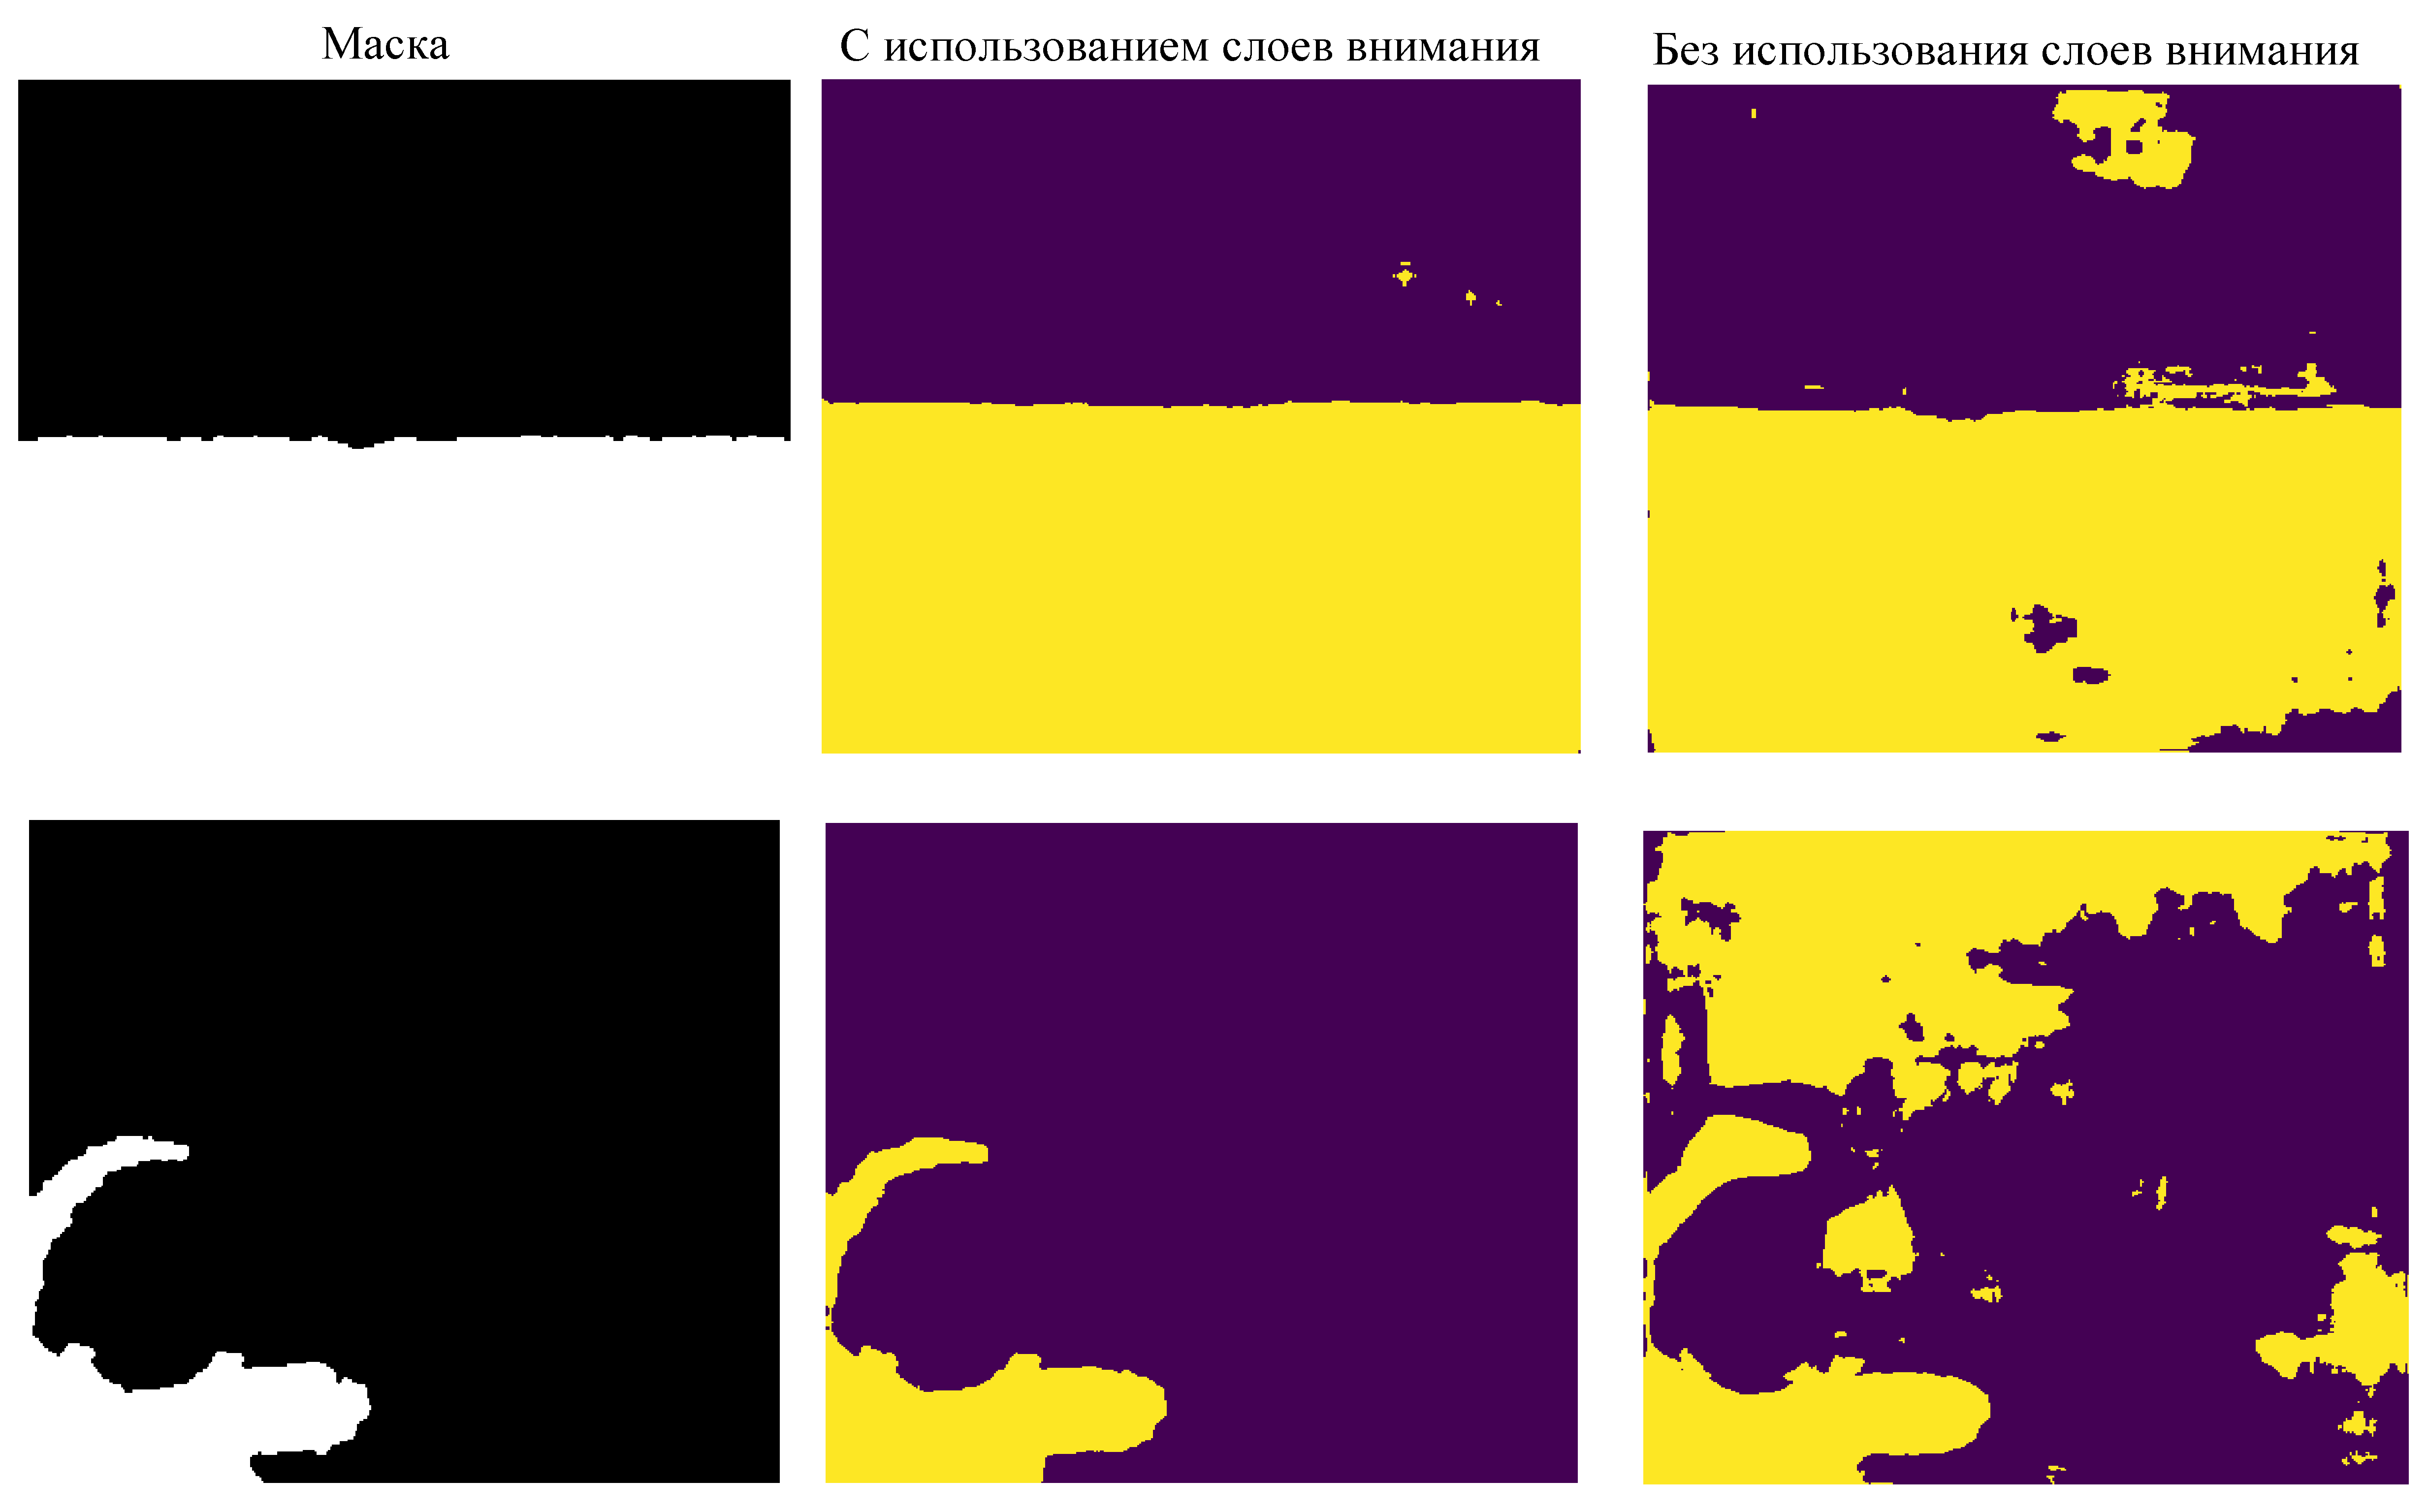
\includegraphics[,scale=0.13]{./img/seam_test.png}
        \caption{Зависимость качества модели от конфигураций слоев внимания.}  
        \label{img:seam1}    
\end{figure}

На основании полученных результатов можно сделать вывод, что добавление слоев внимания приводит к существенному приросту обеих ключевых метрик. Данный результат подтверждает высокую эффективность механизма внимания для задачи обнаружения фальсифицированных фрагментов. Поскольку область подделки обычно занимает малую долю изображения, большинство каналов признаков содержит информацию о нормальном фоне. Без механизма внимания модель «размазывает» внимание по всем каналам, что приводит к высокому уровню ложноположительных срабатываний (FP) и пропуску мелких деталей подделки (FN). Слой внимания позволяет модели фокусироваться на высокочастотных артефактах, характерных для фальсифицированных областей. Это особенно важно при решении задачи сегментации с сильным дисбалансом классов. Таким образом, использование слоев внимания значительно повышает качество модели, делая её более чувствительной к локальным артефактам подделки. 

\section{Влияние слоя адаптации признаков на качество модели}

Целью данного исследования является изучение эффективности использования слоев адаптации признаков в реализованной модели сверточной нейронной сети. 

Для проведения этого исследования было выполнено сравнительное тестирование трёх конфигураций модели: без использования слоев адаптации признаков, со слоями адаптации в виде единых блоков свёртки и со слоями адаптации в виде остаточных блоков. Все остальные компоненты архитектуры оставались неизменными. Эксперимент проводился на одной и той же тестовой выборке. Результаты эксперимента представлены в таблице \ref{tab:fal}.

\begin{table}[H]
    \centering
    \caption{Зависимость точности от конфигураций}\label{tab:fal}
    \begin{tabular}{|p{6cm}|p{4cm}|p{4cm}|}
        \hline
        \textit{Конфигурация} &\centering \textit{{Значение F1}} & \textit{Значение IoU}\\ \hline
        Без использования слоев адаптации признаков &  0.6829 &  0.6011 \\ \hline
        Слои адаптации признаков как единые блоки свёртки & 0.7653 & 0.7139\\ \hline
        Слои адаптации признаков как остаточные блоки & 0.9042 &  0.8252 \\ \hline
    \end{tabular}
\end{table}

Примеры результатов обнаружения модели при различных конфигурациях слоев адаптации признаков представлены на рисунке \ref{img:fal1}.

\captionsetup{justification=centering,singlelinecheck=off}
\begin{figure}[h!]
    \centering
        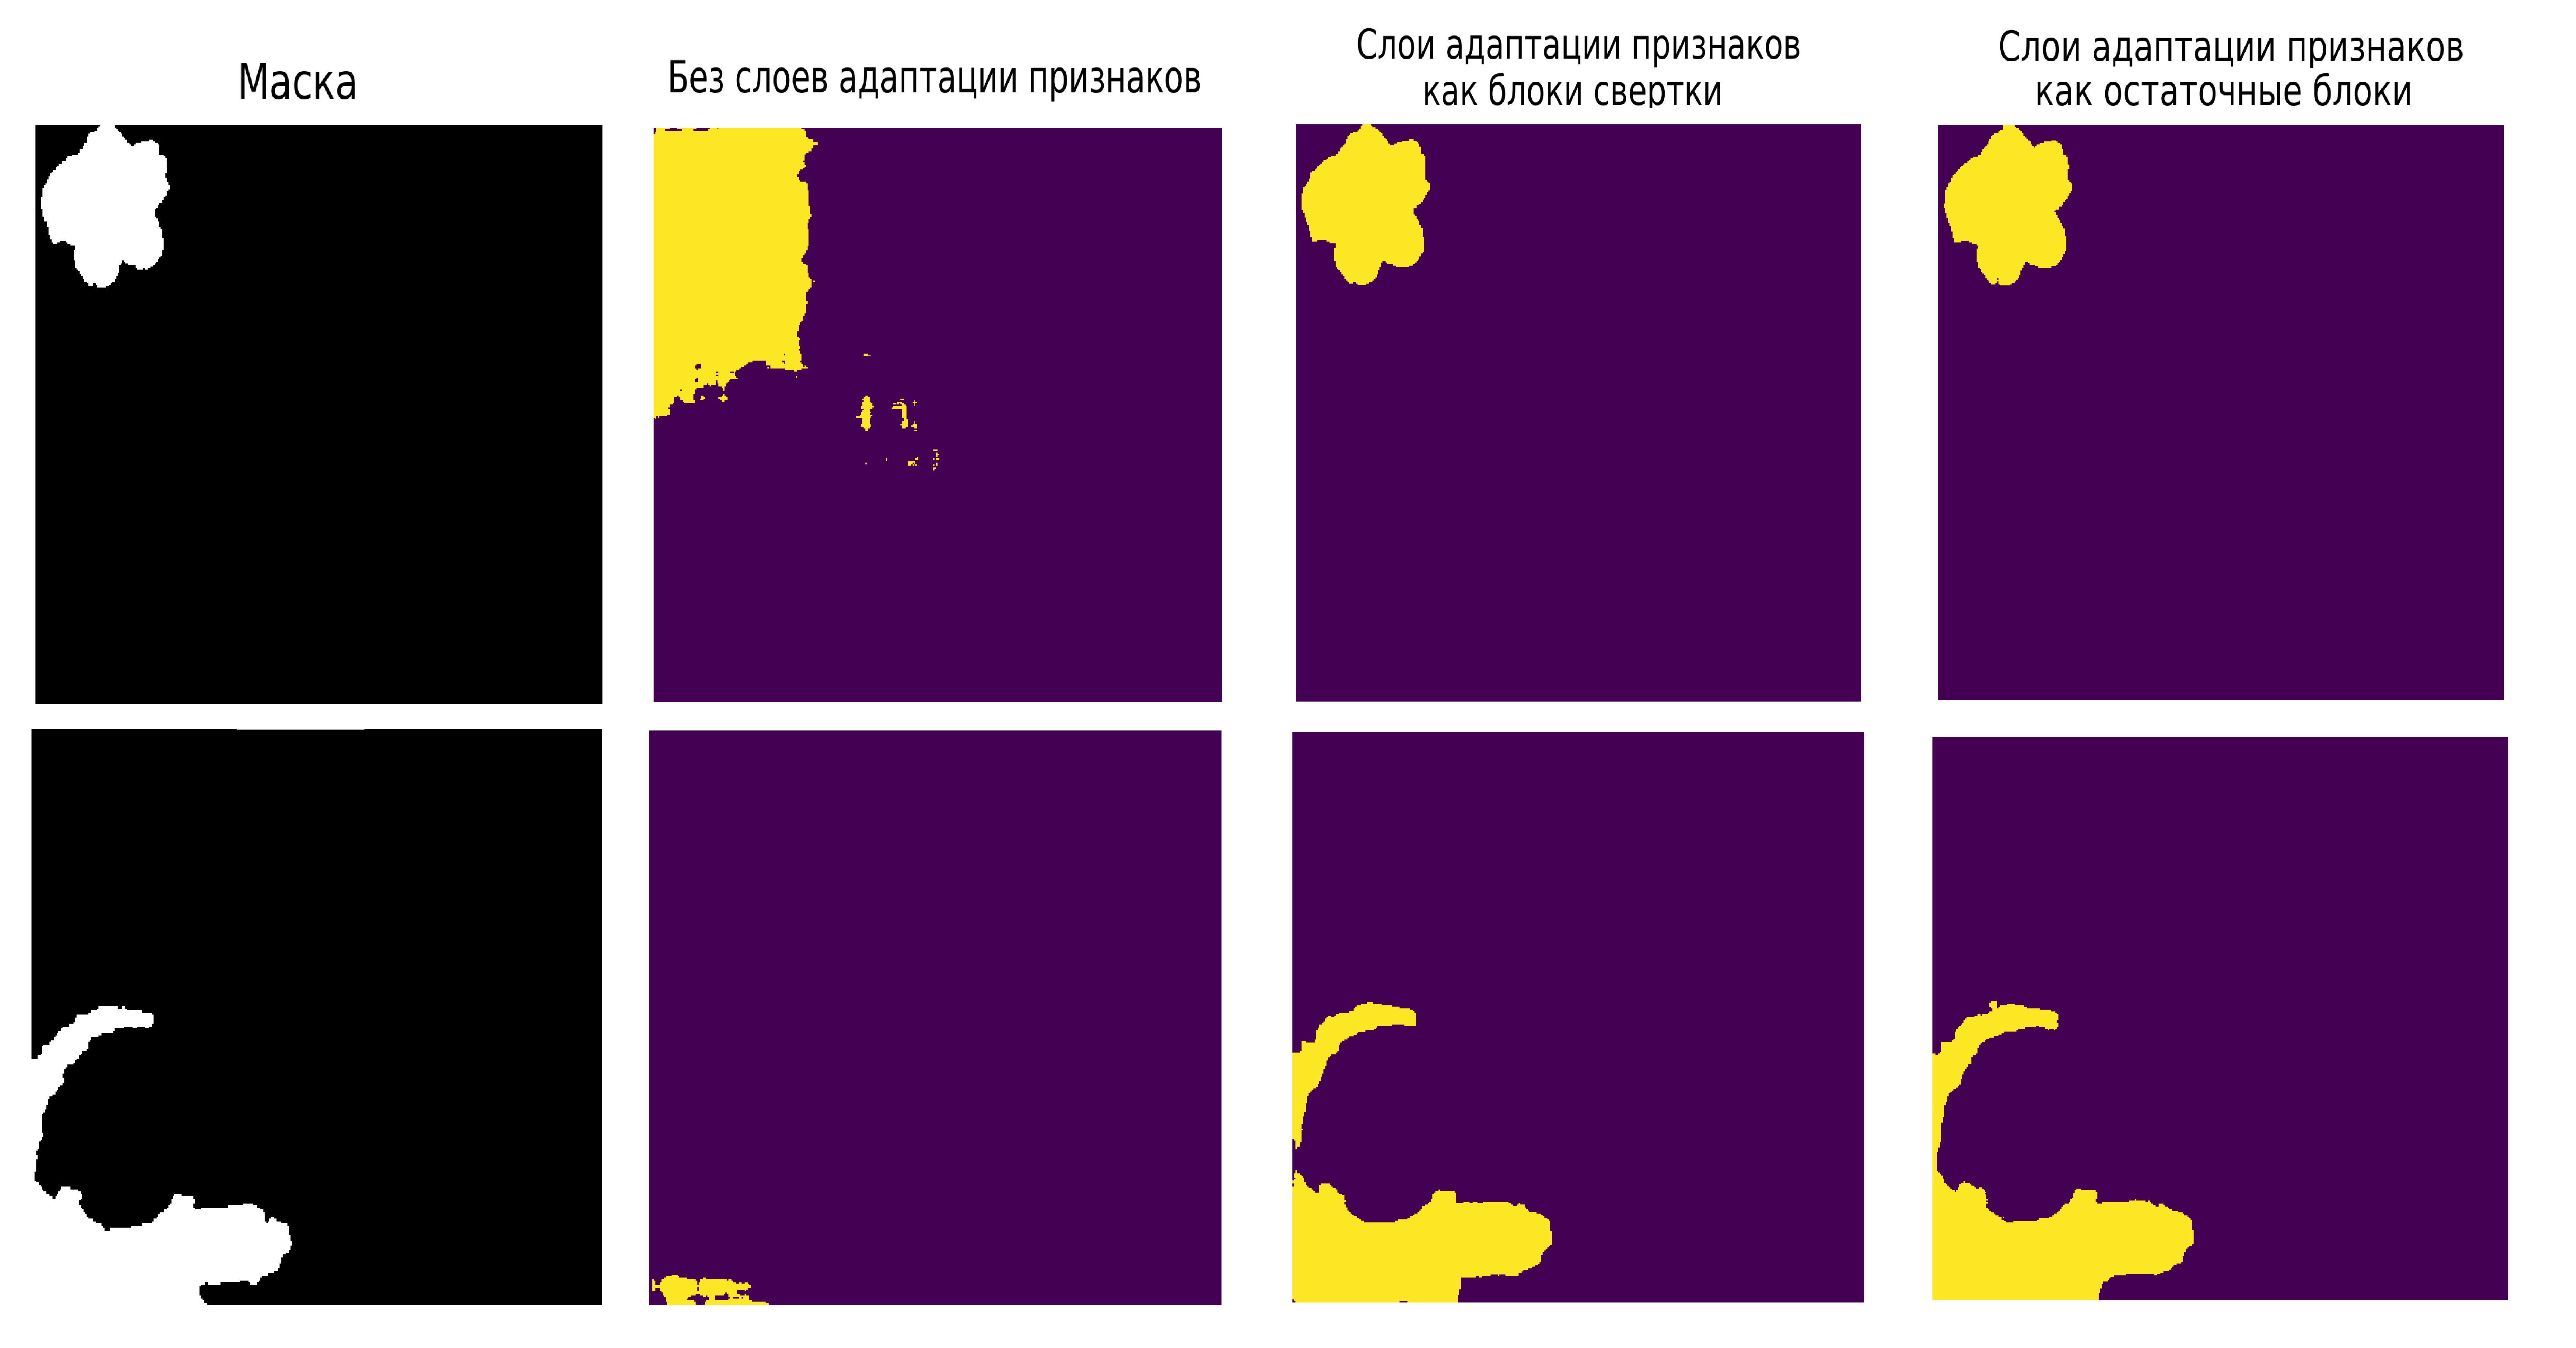
\includegraphics[,scale=0.1]{./img/fal_test.png}
        \caption{Зависимость качества модели от конфигураций слоев адаптации признаков.}  
        \label{img:fal1}
\end{figure}    

На основании полученных результатов можно сделать вывод, что отказ от слоев адаптации признаков приводит к значительному снижению качества, использование простых сверточных блоков даёт умеренное улучшение, наилучшие результаты достигаются при реализации слоев адаптации в виде остаточных блоков. Основная причина такого различия заключается в природе признаков, поступающих из ветви извлечения признаков. Эти признаки содержат высокочастотные детали, которые при прямом объединении с семантическими картами основной ветви создают значительные помехи. Это приводит к размытию границ предсказанной маски и высокому уровню ложноположительных результатов на фоне. При использовании единых сверточных блоков качество улучшается, но всё ещё наблюдается потеря мелких деталей. Остаточные блоки обеспечивают чёткие, точные границы маски и минимальное количество ложных срабатываний даже на сложных текстурах фона. Таким образом, слои адаптации признаков, реализованные в виде остаточных блоков, являются оптимальным решением. Они эффективно фильтруют помехи, сохраняют важную высокочастотную информацию и обеспечивают наилучшее качество локализации фальсифицированных фрагментов при сильном дисбалансе классов.

\section{Влияние объема передаваемых данных на качество работы метода}

Целью данного исследования является изучение зависимости точности метода обнаружения фальсифицированного фрагмента от объема передаваемых данных. Поскольку в рамках используемой архитектуры сверточной нейронной сети основным фактором, определяющим объем обрабатываемой информации, выступает пространственное разрешение входного изображения, в эксперименте рассматривались изображения различных размеров: 384×256, 640×480 и 800×600 пикселей. Большее число пикселей соответствует большему объему данных, поступающих на вход сети.

Тестирование проводилось на единой тестовой выборке. Все компоненты модели, включая слои внимания и адаптации признаков, оставались неизменными. В качестве оцениваемых показателей использовались усредненные по каждой размерной группе значения F1-меры и IoU. Результаты эксперимента представлены ниже в таблице \ref{tab:size}.

\begin{table}[H]
    \centering
    \caption{Зависимость точности от размеров входного изображения}\label{tab:size}
    \begin{tabular}{|p{6cm}|p{4cm}|p{4cm}|}
        \hline
        \textit{Размер изображения} &\centering \textit{{Значение F1}} & \textit{Значение IoU}\\ \hline
        % 256×384 &  0.9356 &  0.8936 \\ \hline
        384×256 & 0.9305 & 0.8887\\ \hline
        640×480 & 0.9270 &  0.8792 \\ \hline
        800×600 & 0.5834 & 0.5190 \\ \hline
    \end{tabular}
\end{table}

На основании полученных результатов можно сделать вывод, что при умеренном объеме передаваемых данных (разрешения 384×256 и 640×480) модель демонстрирует стабильно высокое качество локализации: средняя F1-мера превышает 0,92, а средний IoU — 0,87. Это свидетельствует о том, что в пределах исследованного диапазона, характерного для многих практических сценариев, эффективность метода практически не зависит от объема данных. Однако при переходе к изображениям большего размера 800×600, то есть при значительном увеличении объема передаваемой информации, наблюдается резкое падение обеих метрик: средняя F1-мера снижается до 0,5834, а средний IoU — до 0,5190. Такое ухудшение объясняется тем, что текущая архитектура сети ориентирована на определенный пространственный масштаб признаков, и при избыточном объеме данных высокочастотные артефакты подделки либо маскируются обилием фоновых деталей, либо требуют более глубокого анализа, не обеспеченного существующей конфигурацией.

Таким образом, проведенный эксперимент подтверждает, что реализованный метод сохраняет высокую эффективность для объемов передаваемых данных, соответствующих разрешениям приблизительно до 640×480. Дальнейшее повышение качества на данных большего объема может быть достигнуто путем модификации архитектуры с целью адаптации к высокоразрешающим изображениям.

\section{Влияние качества изображения на качество модели}

Целью данного исследования является изучение влияния качества изображений на точность разработанного метода.

Для проверки устойчивости модели был проведен эксперимент по сжатию входных изображений по стандарту JPEG. Поскольку в реальных условиях изображения часто подвергаются сжатию, важно оценить, как изменение коэффициента качества влияет на точность локализации. Исследование проводилось при варьировании качества от 0.85 до 1, а результаты по метрикам F1-score и IoU представлены на рисунке \ref{img:jpeg}.

\captionsetup{justification=centering,singlelinecheck=off}
\begin{figure}[h!]
	\centering
		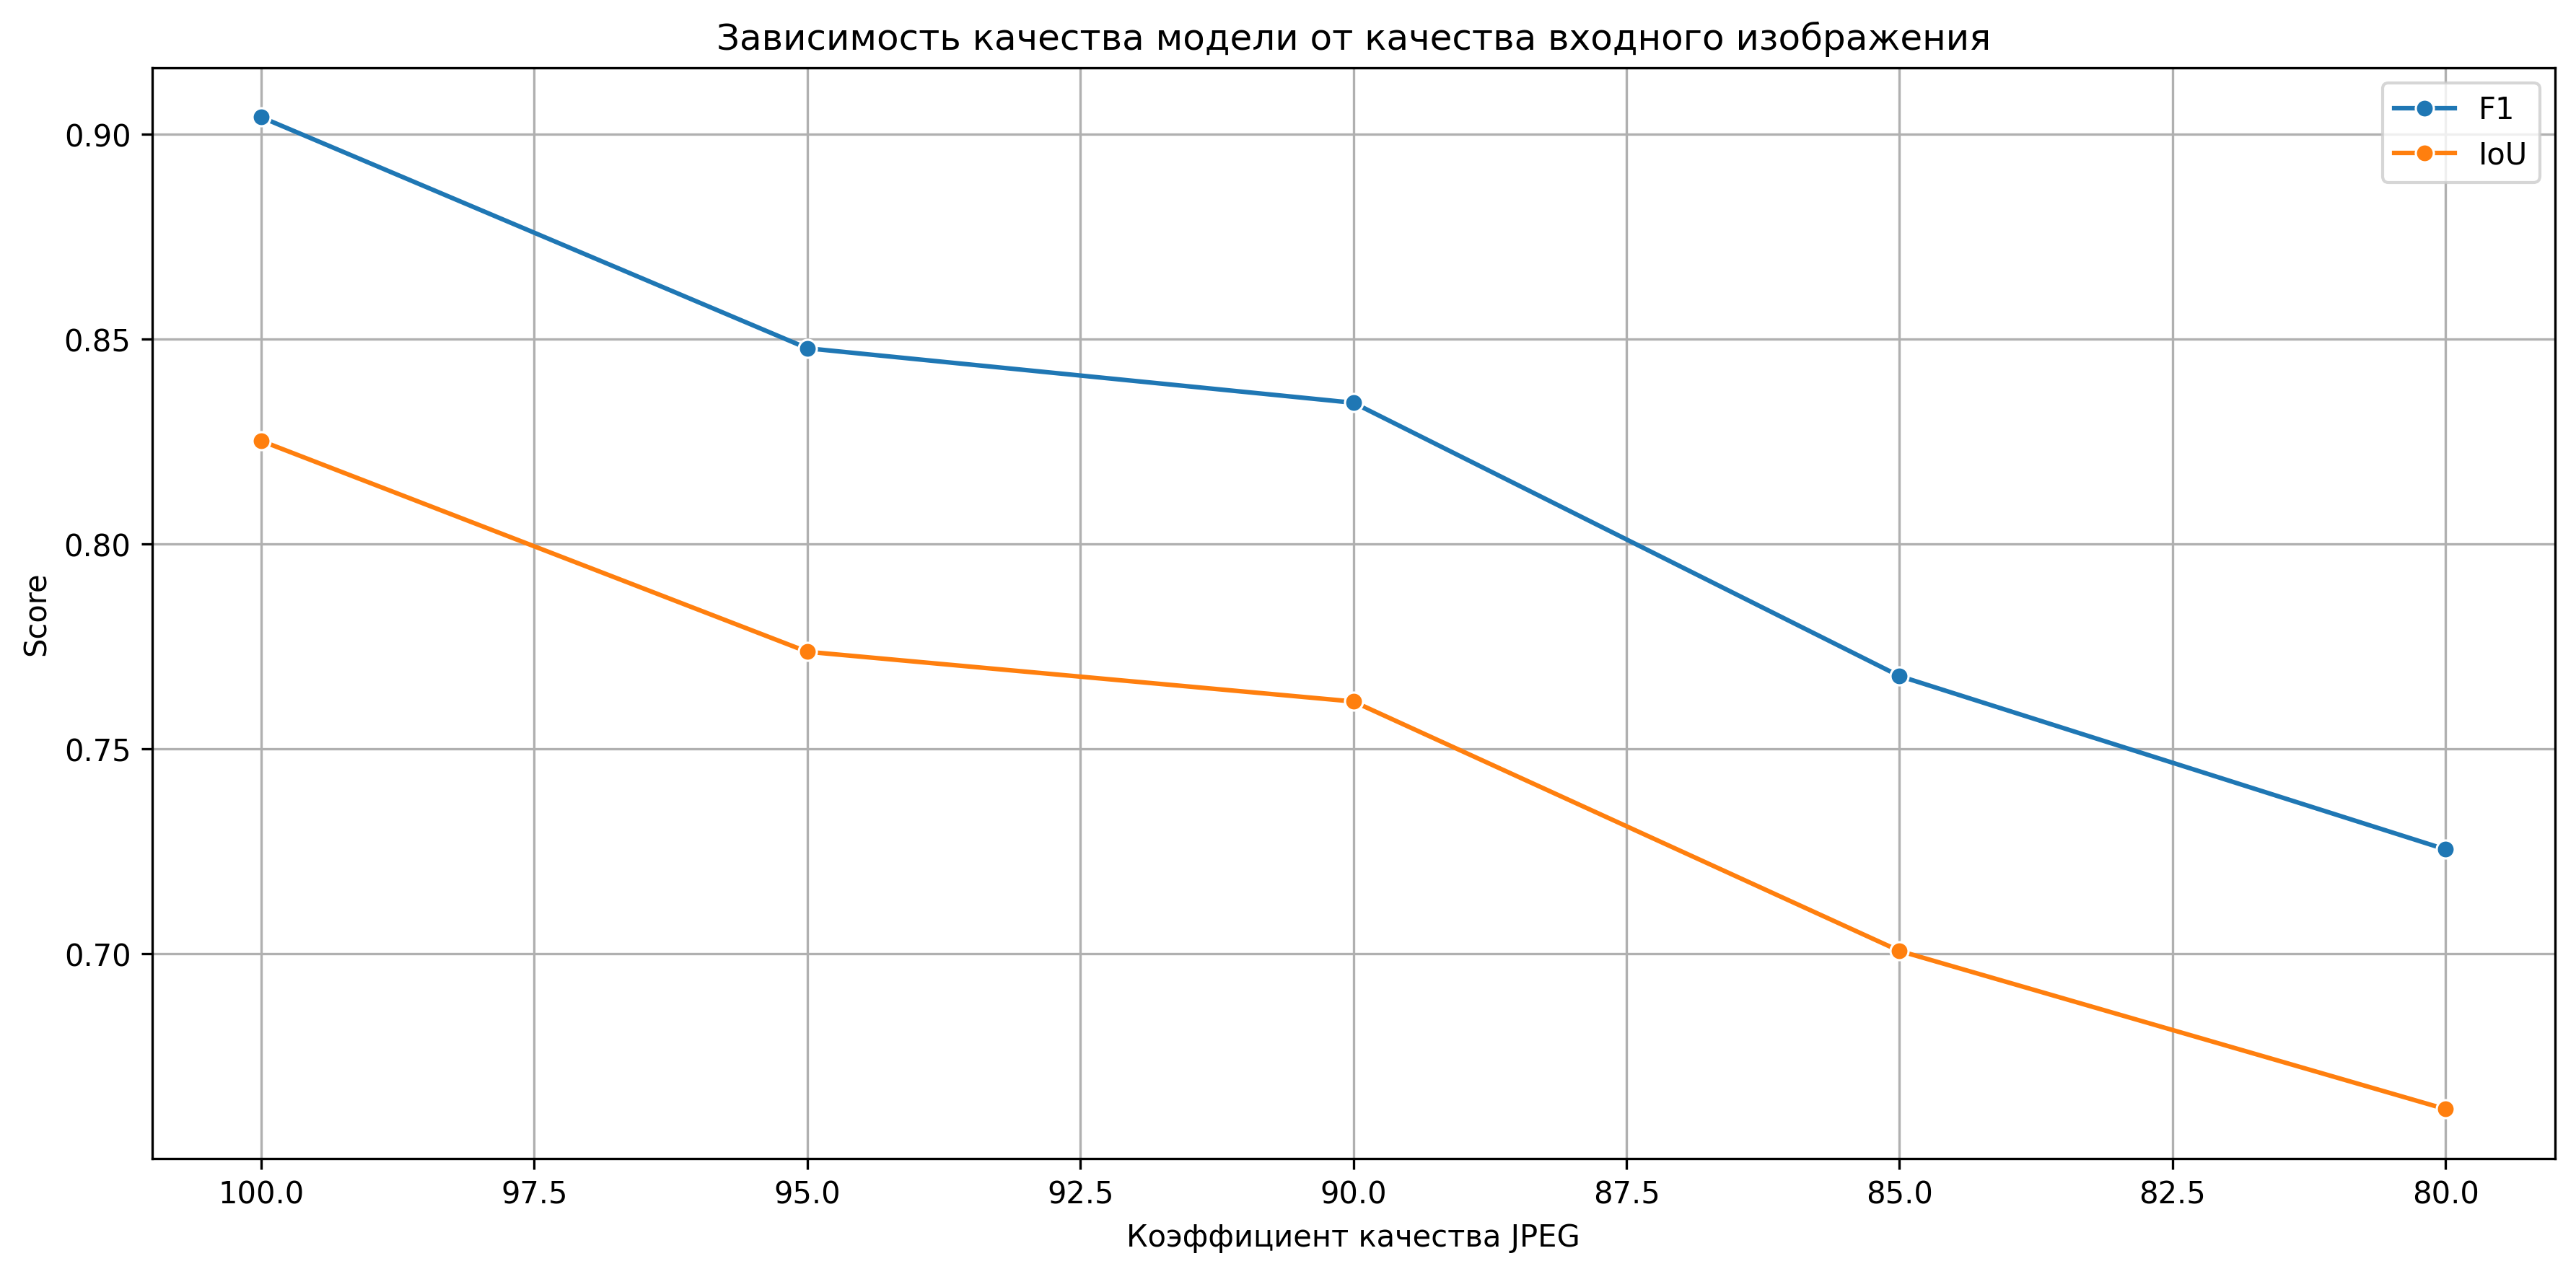
\includegraphics[,scale=0.5]{./img/jpeg.png}
		\caption{Зависимость качества модели от качества изображений.}  
		\label{img:jpeg}
\end{figure}

На основании полученных результатов можно сделать вывод, что точность разработанного метода существенно зависит от уровня сжатия JPEG входного изображения. При высоком качестве изображения (коэффициент JPEG равен 100) модель демонстрирует наилучшие результаты. Однако с увеличением степени сжатия (уменьшением коэффициента качества JPEG) наблюдается устойчивое снижение обеих метрик. Данная зависимость свидетельствует о достаточной чувствительности модели к потерям информации, вызванным JPEG-компрессией, которая является одним из наиболее распространённых видов постобработки в реальных условиях. Тем не менее, даже при сильном сжатии  модель сохраняет приемлемый уровень точности локализации, что подтверждает её определённую робастность. Полученные результаты указывают на необходимость дальнейшего совершенствования архитектуры, в частности, путём введения дополнительных механизмов устойчивости к JPEG-артефактам.

\section*{Вывод}

В ходе исследования разработанной сверточной нейронной сети были выбраны и обоснованы основные метрики оценки качества локализации фальсифицированного фрагмента — F1-мера и IoU. Эксперименты показали, что использование слоя внимания значительно повышает точность модели. Наилучшие результаты достигаются при применении слоёв адаптации признаков в виде остаточных блоков, которые эффективно фильтруют шум и сохраняют важную информацию. Исследование влияния объема передаваемых данных показало стабильные высокие результаты на изображениях разрешений до 640×480 и заметное снижение качества при переходе к большим объемам (800×600). Кроме того, установлено, что качество работы модели сильно зависит от степени сжатия JPEG: при коэффициенте 100 достигаются максимальные значения метрик, однако даже при сильном сжатии (JPEG = 80) модель сохраняет приемлемую точность. Полученные результаты подтверждают эффективность предложенного подхода и указывают на необходимость дальнейшего повышения робастности к постобработке изображений.